\documentclass[tikz,border=12pt]{standalone}
\usepackage{amsmath,amssymb}
\usetikzlibrary{calc,arrows.meta}

\begin{document}
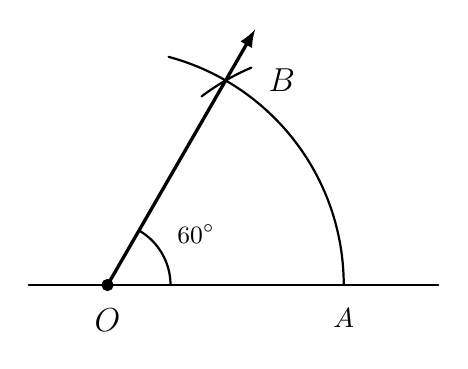
\begin{tikzpicture}[>=latex, line cap=round, line join=round]
  % Parameters
  \def\r{3.0}     % Radius of compass opening

  % Baseline
  \draw[thick] (-1.0, 0) -- (4.2, 0);

  % Vertex O
  \coordinate (O) at (0, 0);
  \filldraw[black] (O) circle (2pt) node[below=5pt, font=\large\bfseries] {$O$};

  % Primary arc centered at O from 0 to 75 degrees
  \draw[thick] (\r, 0) arc (0:75:\r);

  % Base intersection point A
  \coordinate (A) at (\r, 0);
  \node[below=5pt, font=\normalsize] at (A) {$A$};

  % Arc centered at A(r, 0) with radius r cutting primary arc at 60 degrees
  \draw[thick] ($(A) + (113:\r)$) arc (113:127:\r);

  % Intersection point B at 60 degrees placed right of the ray with generous space
  \coordinate (B) at ({\r*cos(60)}, {\r*sin(60)});
  \node[right=12pt, font=\large] at (B) {$B$};

  % Constructed 60-degree ray from O through B
  \draw[very thick, ->] (O) -- ({1.25*\r*cos(60)}, {1.25*\r*sin(60)});

  % 60-degree angle arc and label
  \draw[thick] (0.8, 0) arc (0:60:0.8);
  \node at (30:1.3) [font=\small\bfseries] {$60^\circ$};

\end{tikzpicture}
\end{document}
